\documentclass[12pt,a4paper]{article}
\usepackage[portuges]{babel}
\usepackage{fontspec}
\usepackage{amsmath}
\usepackage{amsfonts}
\usepackage{amssymb}
\usepackage{graphicx}
\usepackage{float}
\author{André Felipe Zanella e Júlia Guizardi}
\title{Implementação do Método de Levenberg-Marquardt}
\date{Outubro, 2022}
\renewcommand\refname{Referências}
\usepackage{setspace}
\usepackage
[boxruled, % Caixa em volta, leg. acima, linha após leg.
linesnumbered, % Numeração das linhas,
portuguese] % Para algoritmos em português.
{algorithm2e}



\newtheorem{teo}{Teorema}[section]
\newtheorem{cor}{Corolário}[teo]
\newtheorem{defi}{Definição}[section]
\newtheorem{lema}[teo]{Lema} 
\newenvironment{dem}[1][Demonstração]{\textbf{#1:}\ } {\hfill\rule{1ex}{1ex}}
\newcounter{ex}[section]
\newenvironment{ex}[1][]{\refstepcounter{ex} \begin{mdframed}[backgroundcolor=white, linewidth=1pt]  \textbf{Exemplo~\theex:} \itshape}
	{\end{mdframed}} 



\begin{document}
	\maketitle
	\section{Introdução}\label{intro}
	Comumente encontramos problemas descritos em sistemas lineares da forma $$Ax = b,$$
	onde $A \in \mathbb{R}^{m\times n},$ $b \in \mathbb{R}^m$ e $x$ é um vetor em $\mathbb{R}^n$ cujo valor deseja-se encontrar.
	Contudo, existem sistemas que não são expressos por equações lineares, chamados sistemas não lineares, iremos abordar uma técnica de resolução deste problema usando o método de Levenberg-Marquardt. Assim, consideremos a função $R: \mathbb{R}^n \longrightarrow \mathbb{R}^m, m\geq n,$ que forma o sistema de equações não lineares descrito por $$R(x)=0.$$
	Sabendo que existe a possibilidade do sistema anterior não possuir solução, queremos minimizar a função objetivo
	\begin{equation}\label{qmnl}
	\min_{x \in \mathbb{R}^{n}} f(x) 
	\\	
	f(x) = \frac{1}{2}||R(x)||^2.
	\end{equation}
	Podemos denotar cada uma das entradas de $r_i:\mathbb{R}^n\longrightarrow \mathbb{R},$ da forma
	$$R(x)=\begin{bmatrix}
	r_1(x)\\ \vdots \\ r_m(x)
	\end{bmatrix}.$$ Com isso, reescrevemos o problema \begin{equation}
	f(x) = \frac{1}{2}\sum_{i=1}^{m}r_i^2(x).
	\end{equation}
	Cada $r_i$ é chamada de função residual.
	
	Definamos $J(x)$ como a matriz jacobiana de $f,$ assim
	\[
	J (x) =
	\begin{bmatrix}
	\frac{\partial{r_i}}{\partial{x_j}}
	\end{bmatrix}
	=
	\begin{bmatrix}
	\nabla r_1(x)^{T} \\
	\nabla r_2(x)^{T} \\
	\vdots \\
	\nabla r_m(x)^{T}
	\end{bmatrix}
	,
	\]

	$1 \leq i \leq m$, $1 \leq j \leq m$.
		
	Desta forma, podemos reescrever a derivada de primeira e segunda ordem da função $f,$ de modo diminuir o custo computacional. Veja,
	
	\[\nabla f(x) = \sum_{i=1}^{m} r_i(x)\nabla r_i(x) = J(x)^{T}r(x)\]
	
	\[\nabla^{2} f(x) = \sum_{i=1}^{m} \nabla r_i(x)\nabla r_i(x)^{T}
	+ \sum_{i=1}^{m} r_i(x) \nabla^{2}r_i(x) = J(x)^{T}J(x) + S(x)\]
	
	com $S(x) = \sum_{i=1}^{m} r_i(x)\nabla^{2}r_i(x).$
	
	Com isso, é necessário o cálculo do vetor gradiente da função $f,$ bem como o produto matricial $(J(x)^{T}J(x)$ e o termo $r_i(x)\nabla^{2}$ para encontrar $S(x).$ Contudo, o valor de $S(x)$ não influência tanto o método quanto o termo que o acompanha, $(J(x)^{T}J(x))$ devido ao valor residual ser pequeno ou ao comportamento próximo ao da função ao redor do ponto de convergência, por isso, muitas vezes podemos desconsiderar seu uso.
	
	\section{Método de Levenberg-Marquardt}\label{lm}
	
	Um dos meios de resolver o problema de quadrados mínimos não lineares é o método de Levenberg - Marquardt. Vamos considerar o problema visto em \ref{qmnl}, e um ponto inicial $x_0,$ assim ao resolver o sistema linear
	 
	\begin{equation*} 
	(J(x_0)^{T}J(x_0) + \lambda_0 I ) d(\lambda_0) = - J(x_0)^T R(x_0),
	\end{equation*}
	sendo $J, R$ já estabelecidos previamente e $\lambda \in \mathbb{R}_+$ o paramêtro que será discutido posteriormente, chamado paramêtro de $damping.$ Vamos encontrar $d(\lambda),$ uma direção mais próxima da solução do problema proposto.
	
	Assim, considerando $x_1 = x_0 + d,$ podemos resolver \ref{sl} continuamente, até encontramos $x_k$ que satisfaça a condição estabelecida.
	
	Veja que este sistema possui solução única, uma vez que a matriz $J^{T}J + \lambda I,$ com $\lambda > 0$ é definida positiva. Portando, o método está bem definido. Além disso, os resultados a seguir garantem o bom funcionamento do método.
	
	\begin{teo}
		Seja $d(\lambda)$ a solução do problema 
		\begin{equation} \label{sl}
		(J(x_k)^{T}J(x_k) + \lambda_k I ) d(\lambda) = - J(x_k)^T R(x_k),
		\end{equation}
		para um valor $\lambda.$ Então, $||d(\lambda)||_2^2$ é uma função contínua decrescente, ou seja, $\lim_{\lambda\rightarrow \infty}{||d(\lambda)||_2^2} = 0.$
	\end{teo}
	
	\begin{teo}
		Seja $\gamma (\lambda)$ o ângulo entre a direção $d(\lambda)$ e a direção máxima de descida. Então, $\gamma(\lambda)$ é uma função contínua monótona decrescente, tal que  $\lim_{\lambda\rightarrow \infty}{\gamma(\lambda)} = 0.$
	\end{teo}

	Note ainda que o método de Levenberg-Maruqardt pode ser entendido como uma evolução do método do gradiente e do método de Gauss-Newton. O método do gradiente consiste na escolha de $d_k$ como sendo a direção $-\nabla f(x_k)$ e a sequência gerada é dada por
	
	\[x_{k+1} = x_k - t \nabla f(x_k)\]
	
	Por outro lado, as direções consideradas pelo método de Gauss - Newton são da forma 
	
	\[ (J(x_k)^{T}J(x_k)d_k = -J^T(x_k)R(x_k). \]
	
	Contudo, o método desenvolvido por Levenberg e melhorado por Marquardt mantém o baixo custo computacional do método de Gauss-Newton e o supera quanto a eficácia de seus iterandos, que estão sempre bem definidos independentemente do problema.
		
	\section{Parâmetro de $Damping$}\label{pd}
	\label{sec:subsec02}
	Para o funcionamento do método resta entender o cálculo de $\lambda,$ conhecido como parâmetro de $damping.$ 
	
	O parâmetro de \textit{damping} é responsável pelo controle da singularidade da matriz $J(x_k)^T J(x_k)$ através da adição de uma matriz diagonal $\lambda_k I$, onde $\lambda_k > 0$ é o parâmetro.
	
	A escolha de um bom parâmetro de \textit{damping} em uma iteração consiste na redução do valor da função objetivo e, simultaneamente garantir que o tamanho do passo tomado não seja muito pequeno, a fim de obtermos a convergência da sequência.
	
	A tabela \ref{tab:damp} apresenta alguns dos parâmetros presentes na literatura.
	
	\begin{table}[H]
		\centering
		\doublespacing
		\begin{doublespace}
		
		\label{tab:damp}
		\begin{tabular}{|c|c|c|}
			\hline
			&\textbf{Parâmetro} & \textbf{Autoria}  \\ \hline
			DP1\label{dp1} & $\lambda_k = \frac{||J(x_k)^T R(x_k)||^{2}_{2}}{f(xk)}$ & Levenberg, \cite{levenberg1944} \\ \hline
			DP2\label{dp2} & $\lambda_k = ||J(x_k)^T R(x_k)||^{2}_{2}$                 & Levenberg modificado, \cite{levenberg1944, benatti2017} \\ \hline
			
			DP3\label{dp3}&$\lambda_k = ||J(x_k)^T R(x_k)||_{2}$                     & Levenberg modificado 2, \cite{levenberg1944, benatti2017}  \\ \hline
			DP4\label{dp4}&$\lambda_k = ||R(x_k)||^{2}_{2} = 2f(x)$                  & Yamashita e Fukushima, \cite{yamashita2001}  \\ \hline
			DP5\label{dp5}&$\lambda_k = ||R(x_k)||_{2} = \sqrt{2f(x)}$               & Fan e Yuan, \cite{fan2001} \\ \hline
		\end{tabular}
		\caption{Alguns parâmetros de $damping.$}
	\end{doublespace}
	\end{table}
	
	Na Seção \ref{testes} iremos abordar o impacto do uso de diferentes parâmetros de $damping,$ inclusive o que ocorre para um valor fixado constante de $\lambda.$ Previamente, vamos estudar a implementação do que já foi discutido na Seção \ref{algoritmo}.
	
	\section{Algoritmo}\label{algoritmo}
	
	A partir da teoria vista nas Seções \ref{lm} e \ref{pd} podemos construir um algoritmo com intuito de resolver \ref{qmnl}. Além do que já foi visto, vamos adicionar a Condição de Armijo, vista no Teorema \ref{ca}, na implementação. Tal condição garante um decréscimo estável, ou seja, proporcional a cada passo que o programa efetua. 
	
	\begin{teo}\label{ca}
		Seja $\alpha \in (0, 1)$ uma constante e $x, d \in \mathbb{R}^n,$ tal que $\nabla f(x) \neq 0$ e ainda, $\nabla f(x)^Td<0.$ Então, existe $\epsilon$ que satisfaz $f(x+td)\leq f(x)+\alpha t\nabla f(x)^Td$ para todo $t \in \left( \left. 0, \epsilon\right] \right..$
	\end{teo}
	
	Assim, podemos estabelecer o Algoritmo \ref{alg} usando o método de Levengerg-Marquardt visto em \cite{aes}.
%\begin{doublespace}
	
	\begin{algorithm}[H] \label{alg}
		\caption{Método de Levenberg-Marquardt com busca linear}
		\textbf{Entrada:} $R(x), J(x), x_0, \alpha \in (0,1)$ e $\epsilon>0$\\
		\textbf{Saída:}: $x^*$ (ponto estacionário) \\
		$k = 0;$\\
		\While {$J(x_k)^TR(x_k) > \epsilon$}{
		Calcule $\lambda_k;$\\
		Obtenha $d(\lambda_k),$ tal que\\ $$(J(x_0)^{T}J(x_0) + \lambda_0 I ) d(\lambda_0) = - J(x_0)^T R(x_0)$$\\
		$t=1;$\\
		\While{$f(x+td)\geq f(x)+\alpha t\nabla f(x)^Td$}{$t = 0.5t$}
		$x_{k+1} = x_k + td(\lambda_k)$\\
		$k = k + 1$
		}
	\end{algorithm}	

%\end{doublespace}
	
	Para garantir a convergência do método é necessário fazermos algumas considerações. Primeiramente, é preciso que a escolha de $\lambda$ seja definido entre constantes positivas. Além disso, para todo $\lambda$ limitado, o ângulo entre a direção de descida do algoritmo e a direção de descida máxima também é limitado por constantes positivas. Por fim, a última hipótese necessária para que o menor autovalor da matriz $J(x)^TJ(x)$ seja limitado superiormente, para qualquer valor que $x$ assumir.
	
	Por fim, resta garantir a convergência do método. 
	
	\begin{lema}
		Consideremos o algoritmo \ref{alg}, satisfazendo todas as hipóteses anteriormente citadas. Portanto, exxistem constantes $\beta > 0$ e $\theta \in (0,1)$ que cumprem
		$$||d(\lambda_k)||_2\geq\beta||\nabla f(x)||_2,$$
		$$\nabla f(x_k)d(\lambda_k)\leq -\theta ||\nabla f(x_k)||_2||d(\lambda_k)||_2.$$
	\end{lema}

	\begin{teo}
		Se $x^*$ é ponto limite da sequência de pontos gerada pelo Algoritmo \ref{alg}, cumprindo as hipóteses anteriormente citadas, então $\nabla f(x^*)=0.$
	\end{teo}

	 Vale a pena citar que o algoritmo implementado neste trabalho, apesar de ter o Algoritmo \ref{alg} como base, não o segue perfeitamente. Primeiramente, nosso algoritmo tem como entrada uma matriz de dados $A,$ e o tipo de função a ser modelada.
	 
	 Com estes dois dados, é possível construir as funções residuais e posteriormente $R,$ bem como a matriz jacobiana $J.$ Além disso, como função auxiliar, foi estabelecido um método de ter como entrada qual parâmetro de $damping$ o usuário deseja utilizar.
	 
 	Além disso, para facilitar o uso do programa, foi acrescentado, com entrada opcional, o vetor gradiente do modelo, tornando facultativo o calculo da derivada pela máquina.
 	
 	Também foi desenvolvido um algoritmo que recebe a matriz de dados e retira os pontos em que ocorre perturbação dos elementos, ou seja, o valor da função residual muito alto, com base na solução disponível para estes testes.
	 	
	 Por fim, foram realizadas algumas implementações que foram de suma importância para a leitura dos dados propostos, bem como os testes que serão analisados na Seção \ref{testes}.
	 
	 Todo o método foi implementado na linguagem \texttt{Julia} e esta disponível online junto a este relatório. 

	Visto isso, é possível aplicarmos o método e desenvolvermos testes capazes de testar sua eficácia na Seção \ref{testes} a seguir.
	
	\section{Testes}\label{testes}
	
	Foi estabelecida uma precisão de $\epsilon = 10^{-10},$ o valor $\alpha = 0.5$ e um número máximo de iterações $k=1000$ para cada conjunto de dados fornecidos.
	
	Os nossos testes foram separados em quatro modelos de funções, sendo eles funções quadráticas(Subseção \ref{quad}), cúbicas (Subseção \ref{cub}), logarítmicas (Subseção \ref{log}) e gaussianas (Subseção \ref{gau}).
	
	\subsection{Função Quadrática}\label{quad}
	Inicialmente, consideramos $x_0 = (1, 0, 0)$ e o parâmetro de $damping$ DP3 em um dos conjuntos de dados a serem analisados pela função quadrática. O resultado do método foi o ponto $x^* = (-1.6568, -6.0813, 0.1420)$ em apenas 14 iterações, quando a solução real do problema era $(-9.5, -8.5, 2.5).$ Veja o resultado na Figura \ref{fig1} (a).
	
	Usamos o programa para tirar a perturbação da matriz de dados e aplicamos no método. Com isso, naturalmente,  obtemos uma solução melhor para o problema e consideravelmente próxima da solução dada. Obtemos, com o parâmetro DP1 o ponto $x^* = (-9.4999, -8.4999, 2.4999)$ em 73 iterações. Observe na Figura \ref{fig1} (b).
	
		\begin{figure}[H]
		\centering 
		\begin{tabular}{ll}
			
			(a)& (b)   \\
			
			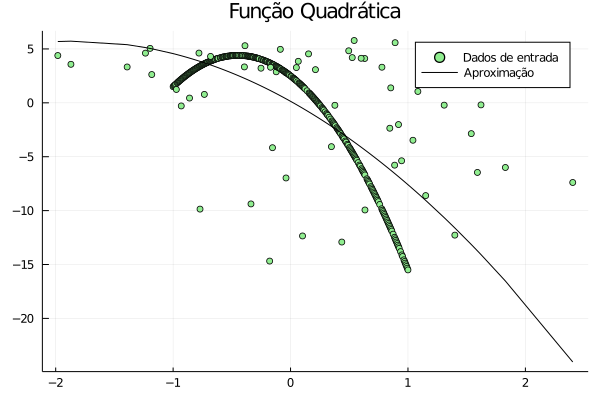
\includegraphics[width=0.45\linewidth]{1.png} & 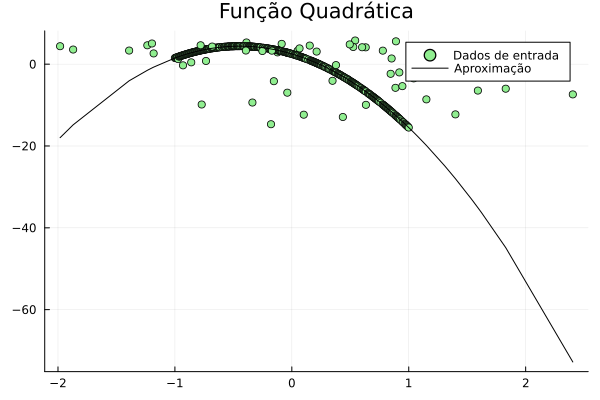
\includegraphics[width=0.45\linewidth]{2.png}\\ 
			
		\end{tabular}
		\caption{Função Quadrática - (a) Aproximação usando todo conjunto de dados. (b) Aproximação feita sem perturbação dos pontos de entrada.}
		\label{fig1}
	\end{figure}


	Ademais, como um teste geral foram avaliados 262 conjuntos de dados com aproximações quadráticas em cada um dos parâmetros, bem como para o valor fixado $\lambda = 0.5.$ O ponto inicial foi $x_0 = (0, 0, 0).$
	
	Sendo avaliado o número médio de iterações para cada conjunto e também a média de erro é definida por $||x^*-sol||,$ onde $sol$ é a solução real do problema.
	
	Foi possível perceber que para os parâmetros DP1, DP3, DP4, DP5 e $0.5$ como valor fixado foi possível encontrar soluções com baixa taxa de erro. Vale a pena destacar que o parâmetro DP1 obteve esse resultado com uma média de poucas iterações, sendo o mais eficiente.
	
	Vale notar que na maioria dos casos a maior diferença entre os resultados obtidos por parâmetros diferentes é o número médio de iterações.
	
	\begin{table}[H]
		\centering
		\begin{tabular}{|c|c|c|}
			\hline
			Parâmetro & Média das iterações & Média do erro\\
			\hline
			
			DP1 & 16.7366 & 3.6247\\
			\hline
			DP2 & 990.9580 & 9.6436\\ \hline
			DP3 & 61.1984 & 3.6247\\ \hline
			DP4 & 837.4847 & 3.5187\\ \hline
			DP5 & 411.5 & 0.6782\\ \hline
			0.5 & 59.4923 & 3.6247\\		\hline	
			
		\end{tabular}
	\end{table}
	\subsection{Função Cúbica} \label{cub}
		Seja $x_0 = (1, 0, 0,0)$ e o parâmetro de $damping$ DP3 em um dos conjuntos de dados a serem analisados pela função cúbica. O resultado do método foi o ponto $x^* = (-0.0517, 3.9730, -9.4655, -3.4345)$ em apenas 34 iterações, quando a solução real do problema era $(0,5,-10,-6).$ Veja o resultado na Figura \ref{fig2} (a).
	
	Vamos realizar os mesmos testes, porém desconsiderando a perturbação. Com o parâmetro $0.5$ obtemos o ponto $x^* = (-4.1319.10^{-14}, 4.9999, -9.9999,$ $ -5.9999)$ em 6 iterações. Observe na Figura \ref{fig2} (b).
	
	\begin{figure}[H]
		\centering 
		\begin{tabular}{ll}
			
			(a)& (b)   \\
			
			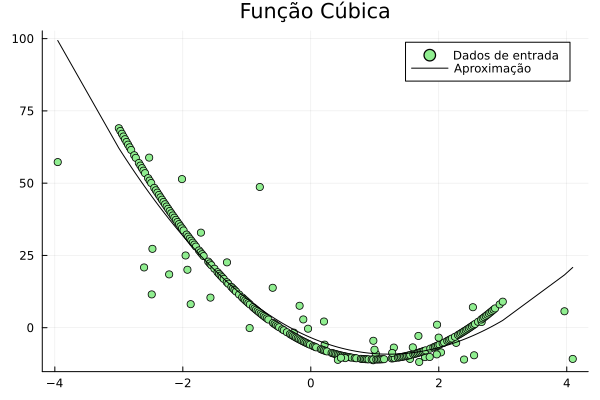
\includegraphics[width=0.45\linewidth]{3.png} & 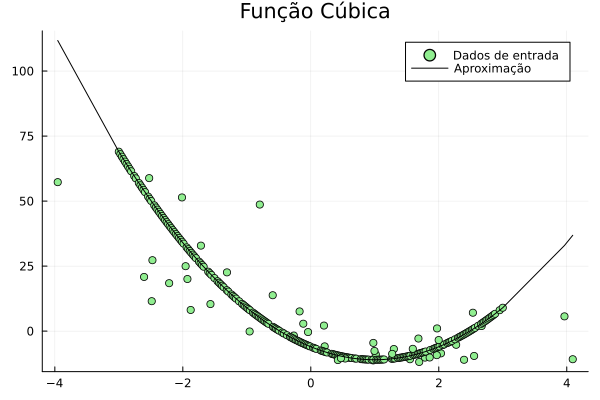
\includegraphics[width=0.45\linewidth]{4.png}\\ 
			
		\end{tabular}
		\caption{Função Cúbica - (a) Aproximação usando todo conjunto de dados. (b) Aproximação feita sem perturbação dos pontos de entrada.}
		\label{fig2}
	\end{figure}
	
	
	Ademais, como um teste geral foram avaliados 252 conjuntos de dados com aproximações cúbicas em cada um dos parâmetros, bem como para o valor fixado $\lambda = 0.5.$ Tomando novamente $x_0 = (0, 0, 0, 0)$ obtivemos um resultado semelhante ao das funções quadráticas, apenas com uma taxa de erro maior. Outra vez, o parâmetro DP1 obteve o mesmo resultado em um número menor de iterações.
	
	Na maioria dos casos a maior diferença entre os resultados obtidos por parâmetros diferentes continua sendo o número médio de iterações.
	
	\begin{table}[H]
		\centering
		\begin{tabular}{|c|c|c|}
			\hline
			Parâmetro & Média das iterações & Média do erro\\
			\hline
			
			DP1 & 13.373 & 13.7759\\
			\hline
			DP2 & 998.8968 & 11.4691\\ \hline
			DP3 & 57.4285 & 13.7759\\ \hline
			DP4 & 953.4047 & 9.5601\\ \hline
			DP5 & 355.623 & 13.7759\\ \hline
			0.5 & 42.1825 & 13.7759\\		\hline	
			
		\end{tabular}
	\end{table}

	\subsection{Função Logarítmica} \label{log}
		Podemos considerar $x_0=(1, 2.5, -5.5)$ e o parâmetro DP3 encontramos o ponto $x^*=(0.7820, 5.9543, -8.6827),$ porém atingiu o número máximo de iterações, 1000.
		
		O resultado pode ser visto na Figura \ref{fig3} (a).
	
	\begin{figure}[H]
		\centering 
		\begin{tabular}{ll}
			
			(a)& (b)   \\
			
			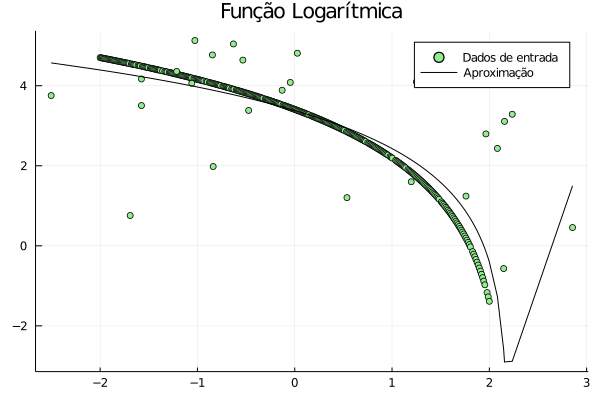
\includegraphics[width=0.45\linewidth]{5.png} & 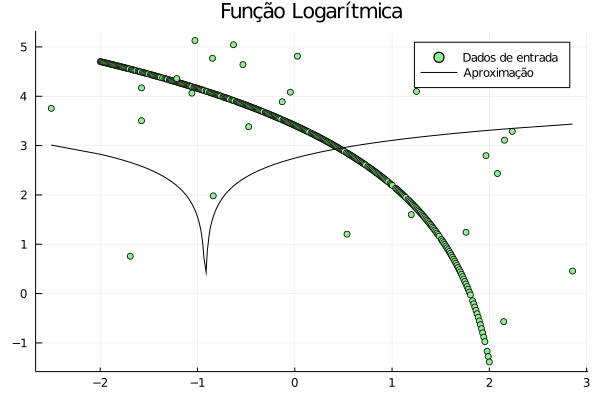
\includegraphics[width=0.45\linewidth]{6.png}\\ 
			
		\end{tabular}
		\caption{Função Logarítmica - (a) Aproximação usando todo conjunto de dados. (b) Aproximação feita sem perturbação dos pontos de entrada.}
		\label{fig3}
	\end{figure}
	
	
	Foram consideradas apenas 10 conjuntos de dados para os testes. O ponto inicial considerado foi $x_0 = (1, 10, 10).$ A função logarítmica obteve resultado com um número bem maior de iterações. Contudo, mais uma vez, o parâmetro DP1 foi o que obteve maior sucesso, e o que vale destacar foi a média do erro, que foi bem menor comparado aos outros parâmetros.
	
	\begin{table}[H]
		\centering
		\begin{tabular}{|c|c|c|}
			\hline
			Parâmetro & Média das iterações & Média do erro\\
			\hline
			
			DP1 & 627.8 & 6.6983\\
			\hline
			DP2 & 900 & 17.3617\\ \hline
			DP3 & 820.6 & 160.8291\\ \hline
			DP4 & 900 & 19.7859\\ \hline
			DP5 & 816.1 & 45.7833\\ \hline
			0.5 & 740.5 & 11.3073\\		\hline	
			
		\end{tabular}
	\end{table}

	\subsection{Função Gaussiana} \label{gau}
	Apliquemos o método em uma função gaussiana. Seja $x_0 = (1, 10, 10)$ e o parâmetro de $damping$ DP3, obtivemos o ponto $x^* = (-4.5002, -2.9811,7.0802)$ em apenas 61 iterações, e a solução do problema é $(-4.5, -3, -7).$ Veja o resultado na Figura \ref{fig4} (a).
	
	Sem a perturbação e com o parâmetro $0.5,$ encontramos o ponto $x^* = (-4.5,-3, 7)$ em 76 iterações. Observe na Figura \ref{fig4} (b).
	
	\begin{figure}[H]
		\centering 
		\begin{tabular}{ll}
			
			(a)& (b)   \\
			
			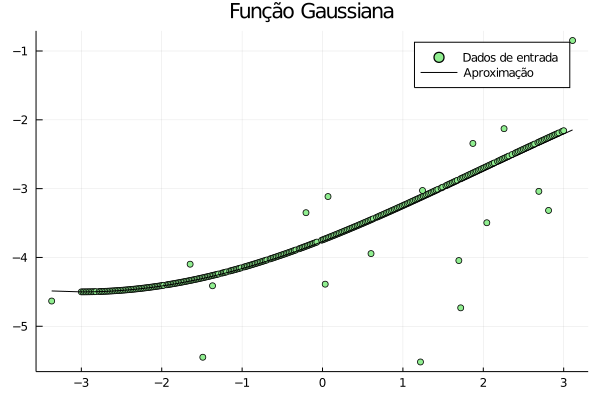
\includegraphics[width=0.45\linewidth]{7.png} & 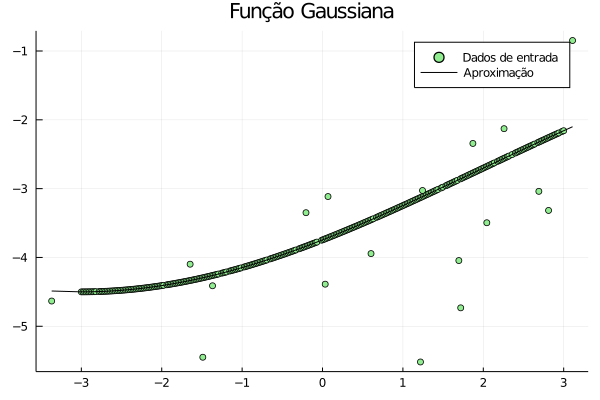
\includegraphics[width=0.45\linewidth]{8.png}\\ 
			
		\end{tabular}
		\caption{Função Gaussiana - (a) Aproximação usando todo conjunto de dados. (b) Aproximação feita sem perturbação dos pontos de entrada.}
		\label{fig4}
	\end{figure}
	
	
	Aqui utilizamos o ponto de entrada $x_0 = (1, 10, 10).$ A função gaussiana obteve o melhor resultado para o parâmetro fixado como $0.5,$ apesar de não ter sido o menor número de iterações, foi encontrado uma média de erro melhor comparado aos outros parâmetros. Percebemos também que para os parâmetros DP4 e DP5 atingimos o número máximo de iterações, apesar disso, ele ainda obteve um erro menor que o encontrado em DP3.
	
	\begin{table}[H]
		\centering
		\begin{tabular}{|c|c|c|}
			\hline
			Parâmetro & Média das iterações & Média do erro\\
			\hline
			
			DP3 & 445.5 & 80.5061\\ \hline
			DP4 & 1000 & 15.0798\\ \hline
			DP5 & 1000 & 13.4543\\ \hline
			0.5 & 797.5 & 9.8600\\		\hline	
			
		\end{tabular}
	\end{table}

	
	\section{Conclusão}
	
	O foco deste trabalho foi uma implementação eficaz do algoritmo gerado pelo método de Levenberg-Marquardt para o problema de quadrados mínimos não linear. Uma vez que tal problema tem grande aplicabilidade em diversar áreas do conhecimento. 
	
	Inicialmente, na Seção \ref{intro} apresentamos o problema a ser estudado, descrito por 
	\begin{equation*}
	\min_{x \in \mathbb{R}^{n}} f(x) 
	\\	
	f(x) = \frac{1}{2}||R(x)||^2.
	\end{equation*}
	
	A seguir, na Seção \ref{lm} vimos a abordagem proposta por Levenberg e aprimorada por Marquardt para resolver tal problema. Dando consequência, estudamos o parâmetro de $damping,$ que pudemos observar pelos resulados vistos na Seção \ref{testes} possui grande influência no resultado encontrado pelo algoritmo abordado na Seção \ref{algoritmo}, principalmente em relação ao número de iterações necessárias para a convergência do método.
	
	Por fim, vale destacar que pudemos comprovar a boa convergência do método em muitos casos, além de expor resultados numéricos do uso do algoritmo.
	
	
	\nocite{aes}
	\nocite{friedlander1994elementos}
	\nocite{kab}
	
	\bibliographystyle{acm}
	\bibliography{ref}

\end{document}